\documentclass[11pt,a4paper]{article}
\usepackage[czech]{babel}
\usepackage[utf8x]{inputenc}
\usepackage[left=2cm,text={17cm, 24cm},top=3cm,a4paper]{geometry}

\usepackage[IL2]{fontenc}
\usepackage{times}
\usepackage[ruled,czech,procnumbered]{algorithm2e}
\usepackage{algorithmic}
\usepackage{multirow}
\usepackage{graphicx}
\usepackage{pdflscape}
\usepackage{marginnote}
\usepackage{listings}
\usepackage{tikz}
\usepackage{pict2e}

\begin{document}


\begin{titlepage}
\begin{center}
\textsc{\Huge Vysoké učení technické v~Brně\\ \medskip
\huge Fakulta informačních technologií}\\
\vspace{\stretch{0.382}}
\LARGE Typografie a publikování\,--\,3. projekt\\
\Huge Tabulky a obrázky\\
\vspace{\stretch{0.618}}
\Large 21.března 2018 \hfill         Maroš Orsák \newpage
\end{center}
\end{titlepage}

\newpage


\section{Úvodní strana}

Název práce umístněte do zlatého řezu a nezapomeňte uvést dnešní datum a vaše jméno a příjmení.


\section{Tabulky}

Pro sázení tabulek můžeme použít buď prostředí \texttt{tabbing} nebo prostředí \texttt{tabular}.

\subsection{Prostředí\texttt{ tabbing}}

Při použití \verb|tabbing| vypadá tabulka následkovně:


% PROSTREDIE TABBING

\begin{tabbing}
	\verb|\pushtabs| \qquad \= \textbf{Cena} \quad\= \kill
	\textbf{Ovoce} \> \textbf{Cena} \> \textbf{Množství} \\
	Jablka\> 			25,90\> 			3 kg\\
	Hrušky\> 			27,40\> 			2,5 kg\\
	Vodní melouny\> 	35,-- \> 			1 kus\\
\end{tabbing}
Toto prostředí se dá také použít pro sázení algoritmů, ovšem vhodnější je použít prostředí \texttt{algorithm} nebo
\texttt{algorithm2e} (viz sekce 3).

% PROSTREDIE TABULAR

\subsection{Prostředí \texttt{ tabular}}

Další možností, jak vytvořit tabulku, je použít prostředí \texttt{tabular}.Tabulky pak budou vypadat takto\footnote{Kdyby byl problem s~\texttt{cline}, zkuste se podívat třeba sem: http://www.abclinuxu.cz/tex/poradna/show/325037.}:

\bigbreak
% JEDNODUCHA TABULKA

\begin{table}[ht]
	\catcode`\-=12
 		\begin{center}
  			\begin{tabular}{|c|c|c|} \hline
     			& \multicolumn{2}{c|}{\textbf{Cena}} \\ \cline{2-3}
   			 	\textbf{Měna} & \textbf{nákup} & \textbf{prodej} \\ \hline 
    			EUR & 27,02 & 27,20 \\
    			GBP & 31,08 & 31,80 \\
    			USD & 25,15 & 25,51 \\ \hline
  			\end{tabular}
  			\caption{Tabulka kurzů k~dnešnímu dni}
			\label{tabulka_1} 		
 		\end{center}
\end{table}

% ZLOZITA TABULKA (viacero tabuliek vedla seba)

\begin{table}[ht] 
	\catcode`\-=12 	
	\begin{center}	
		%PRVA DVOJ-STLPCOVA TABULKA |C|C|
		\begin{tabular}{|c|c|}            \hline
			$A$ & $\neg A$\\ 			  \hline
			$\textbf{P}$ & N\\ \hline
			$\textbf{O}$ & O\\ \hline
			$\textbf{X}$ & X\\ \hline
			$\textbf{N}$ & P\\
			\hline
		\end{tabular}
		%DRUHA 6-STLPCOVA TABULKA |C|C|C|C|C|C|
		\begin{tabular}{|c|c|c|c|c|c|} \hline
			\multicolumn{2}{|l|}{\multirow{2}{*}{$A \wedge B$}} 
				& \multicolumn{4}{c|}{$B$}  \\ \cline{3-6} 
				\multicolumn{2}{|c|}{} 
					& \textbf{P} & \textbf{O} & \textbf{X} & \textbf{N} \\ \hline
					\multirow{4}{*}{$A$}
						& \textbf{P} & P & O~& X & N \\ \cline{2-6} 
						& \textbf{O} & O~& O~& N & N \\ \cline{2-6}  
 						& \textbf{X} & X & N & X & N \\ \cline{2-6} 
 						& \textbf{N} & N & N & N & N \\ \hline 
		\end{tabular}
		%TRETIA 6-STLPCOVA TABULKA |C|C|C|C|C|C|				
		\begin{tabular}{|c|c|c|c|c|c|} \hline
			\multicolumn{2}{|l|}{\multirow{2}{*}{$A \vee B$}} 
				& \multicolumn{4}{c|}{$B$}  \\ \cline{3-6} 
				\multicolumn{2}{|c|}{} 
					& \textbf{P} & \textbf{O} & \textbf{X} & \textbf{N} \\ \hline
					\multirow{4}{*}{$A$} 
						& \textbf{P} & P & P & P & P \\ \cline{2-6} 
 						& \textbf{O} & P & O~& P & O~\\ \cline{2-6}  
 						& \textbf{X} & P & P & X & X \\ \cline{2-6} 
 						& \textbf{N} & P & O~& X & N \\ \hline 
	 	\end{tabular}
		%STVRTA 6-STLPCOVA TABULKA |C|C|C|C|C|C|
		\begin{tabular}{|c|c|c|c|c|c|} \hline
			\multicolumn{2}{|l|}{\multirow{2}{*}{$A \rightarrow B$}} 
				& \multicolumn{4}{c|}{$B$}  \\ \cline{3-6} 
				\multicolumn{2}{|c|}{} 
					& \textbf{P} & \textbf{O} & \textbf{X} & \textbf{N} \\ \hline
					\multirow{4}{*}{$A$} 
						& \textbf{P} & P & O~& X & N \\ \cline{2-6} 
 						& \textbf{O} & P & O~& P & O~\\ \cline{2-6}  
 						& \textbf{X} & P & P & X & X \\ \cline{2-6} 
 						& \textbf{N} & P & P & P & P \\ \hline 
		\end{tabular}
		\caption{Protože Kleeneho trojhodnotová logika už je \uv{zastaralá}, uvádíme si zde příklad čtyřhodnotové
logiky}
	\label{tabulka_2}
	\end{center}
\end{table}



\section{Algoritmy}

Pokud budeme chtít vysázet algoritmus, můžeme použít prostředí \texttt{algoritm}\footnote{Pro nápovědu, jak zacházet s~prostředím \texttt{algorithm},můžeme zkusit tuhle stránku: \\ http://ftp.cstug.cz/pub/tex/CTAN/macros/latex/contrib/algorithms/algorithms.pdf.} nebo \texttt{algorithm2e}\footnote{Pro \texttt{algorithm2e } zase tuhle: http://ftp.cstug.cz/pub/tex/CTAN/macros/latex/contrib/algorithm2e/algorithm2e.pdf.}. Příklad použití prostrědí \texttt{algorithm2e} viz Algoritmus 1.

% ALGORITMUS...

\begin{algorithm}
	\label{algoritmus}
	\sloppy
	\caption{\textsc{Fast}SLAM}
	\SetKwHangingKw{Input}{Input:}
	\SetKwHangingKw{Output}{Output:}
	\DontPrintSemicolon
	\Input{$(X_{t-1},u_t,z_t)$}
	\Output{$X_t$}
	\begin{algorithmic}[1]  
		\STATE $\overline{X_t}=X_t=0$
		\FOR{$k = 1$ to $M$}
    		\STATE ${x_t}^{[k]}=sample\_motion\_model(u_t,x_{t-1}^{[k]})$
    		\STATE ${\omega_t}^{[k]}=measurement\_model(z_t,x_t^{[k]},m_{t-1})$
    		\STATE ${m_t}^{[k]}=updated\_occupancy\_grid(z_t,x_{t}^{[k]},m_{t-1}^{[k]})$
    		\STATE $\overline{X_t}=\overline{X_t} +\langle x_x^{[m]}, \omega_t^{[m]}\rangle$
		\ENDFOR
		\FOR{$k = 1$ to $M$}
    		\STATE draw $i$ with probability $ \approx \omega_t^{[i]}$
    		\STATE add $\langle x_x^{[k]},m_t^{[k]}\rangle $ to $X_t$
		\ENDFOR
		\RETURN $X_t$ 
	\end{algorithmic} 
\end{algorithm}


\section{Obrázky}

Do našich  můžeme samozřejmě vkládat obrázky. Pokud je obrákem fotografie, můžeme klidně použít bitmapový soubor. Pokud by to ale mělo být nějaké schéma nebo něco podobného, je dobrým zvykem takovýto obrázek vytvořit vektorově.

% OBRAZOK C.1

\begin{figure}[htb]
 	\centering
 		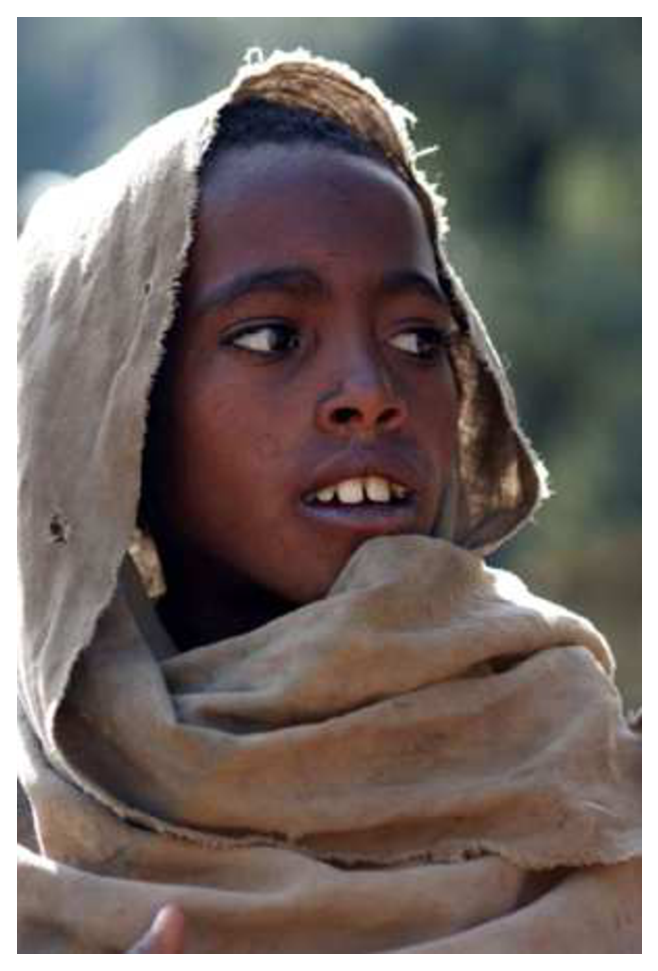
\includegraphics[scale=0.43]{etiopan.eps}
 		\reflectbox{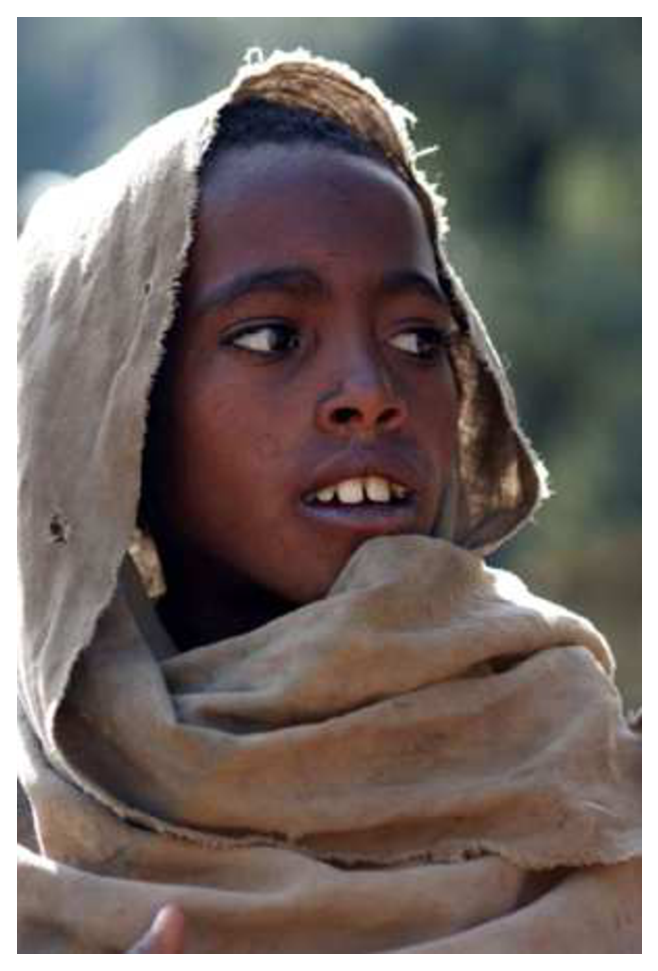
\includegraphics[scale=0.43]{etiopan.eps}}
 		\caption{Malý etiopánek a jeho bratříček}
 		\label{Picture1}
\end{figure}

\newpage

Rozdíl mezi vektorovým \dots

% OBRAZOK C.2

\begin{figure}[htb]
 	\centering
 		
\includegraphics[scale=0.43]{oniisan.eps}
 		\caption{Vektorový obrázek}
 		\label{Picture2}
\end{figure}

\bigbreak

\dots a bitmapovým obrázkem


% OBRAZOK C.3

\begin{figure}[htb]
 	\centering
 		
\includegraphics[scale=0.65]{oniisan2.eps}
 		\caption{Bitmapový obrázek}
 		\label{Picture3}
\end{figure}

\bigbreak

\noindent se projeví například při zvětšení.

Odkazy (nejen ty) na obrázky \ref{Picture1},\ref{Picture2} a \ref{Picture3}, na tabulky \ref{tabulka_1} a \ref{tabulka_2} a také na algoritmus \ref{algoritmus} jsou udělány pomocí křížových odkazů. Pak je ovšem potřeba zdrojový soubor přeložit dvakrát.

Vektorové obrázky lze vytvořit i přímo v~\LaTeX u, například pomocí prostředí \texttt{picture}.  

\newpage

\begin{landscape}
	\thicklines
	\setlength{\unitlength}{1cm}
	\centering	
	\begin{picture}(24,11)

	% ZAKLADNA HRANA PODSTAVA
	\linethickness{6pt}
	\put(2.5,2){\line(1,0){19}}	
	
	% KRUH 	
	\linethickness{1pt}
	\put(19.5,8.5){\circle{2.01}}	
	
	\linethickness{2pt}
	\put(5,2){\line(0,1){4}}
	\put(5,6){\line(1,0){5}}
	
	%%1.OBDLZNIK ZACIATOK (MALY)
	\put(10,6){\line(0,1){0.5}}
	\put(10,6){\line(0,-1){0.5}}
	\put(10,6.5){\line(1,0){4}}
	\put(10,5.5){\line(1,0){4}}
	\put(14,5.5){\line(0,1){1}}	
	%%1.OBDLZNIK KONIEC   (MALY)
	
	\put(14,5.7){\line(1,0){4}}
	\put(18,5.7){\line(0,-1){0.2}}
	
	%%2.OBDLZNIK ZACIATOK (VELKY)
	\put(19,5.5){\line(-1,0){5}}
	\put(10,5.5){\line(-1,0){2.5}}
	\put(7.5,5.5){\line(0,-1){0.8}}
	\put(7.5,4.7){\line(1,0){11.5}}
	\put(19,4.7){\line(0,1){0.8}}
	%%2.OBDLZNIK KONIEC   (VELKY)
	
	\put(7.5,4.7){\line(1,-1){1.25}}
	\put(6.25,3.45){\line(1,0){4}}
	\put(6.25,3.45){\line(0,-1){1.45}}
	\put(10.25,3.45){\line(2,-1){2.9}}
	%3.OBDLZNIK ZACIATOK
	\put(10.5,3.3){\line(0,1){1.25}}
	\put(10.5,4.55){\line(1,0){8.25}}
	\put(18.75,4.55){\line(0,-1){1.5}}
	\put(18.75,3.05){\line(-1,0){7.7}}	
	%3.OBDLZNIK KONIEC
	
	\put(18.75,3.05){\line(1,0){0.4}}
	\put(19.15,3.05){\line(0,-1){1.05}}	

	\linethickness{2pt}
	\put(2,0){\framebox(20,10){}}

\end{picture}

\bigbreak

Obrázek 4: Vektorový obrázek
\label{Picture4}
\end{landscape}



\end{document}
